\documentclass[conference]{IEEEtran}
\IEEEoverridecommandlockouts
% The preceding line is only needed to identify funding in the first footnote. If that is unneeded, please comment it out.
\usepackage{cite}
\usepackage{amsmath,amssymb,amsfonts}
\usepackage{algorithmic}
\usepackage{graphicx}
\usepackage{textcomp}
\usepackage{xcolor}
\def\BibTeX{{\rm B\kern-.05em{\sc i\kern-.025em b}\kern-.08em
    T\kern-.1667em\lower.7ex\hbox{E}\kern-.125emX}}
\begin{document}

\title{Scholarium \\
{\footnotesize \textsuperscript * A safe and innovative way to manage diploma issuing and verification}
\thanks{}
}

\author{\IEEEauthorblockN{1\textsuperscript{st} Dascalu Stefan}
\IEEEauthorblockA{\textit{Student Sergent Major } \\
\textit{Academia Tehnică Militară}\\
București, Romania \\
st3fandascalu@gmail.com}
\and
\IEEEauthorblockN{2\textsuperscript{nd} Avram Andrei Marius}
\IEEEauthorblockA{\textit{Student Sergent Major} \\
\textit{Academia Tehnică Militară}\\
București, Romania \\
avram.andreimarius@gmail.com}
\and
\IEEEauthorblockN{3\textsuperscript{rd} Given Name Surname}
\IEEEauthorblockA{\textit{dept. name of organization (of Aff.)} \\
\textit{name of organization (of Aff.)}\\
City, Country \\
email address}
\and
\IEEEauthorblockN{4\textsuperscript{th} Given Name Surname}
\IEEEauthorblockA{\textit{dept. name of organization (of Aff.)} \\
\textit{name of organization (of Aff.)}\\
City, Country \\
email address}
\and
\IEEEauthorblockN{5\textsuperscript{th} Given Name Surname}
\IEEEauthorblockA{\textit{dept. name of organization (of Aff.)} \\
\textit{name of organization (of Aff.)}\\
City, Country \\
email address}

}

\maketitle

\begin{abstract}
There are numerous websites that facilitate a way to purchase a diploma. Also there are multiple institutions that practice the handling of diplomas in ways that are not transparent to the receiving entities or those that accreditate the institution node. In accordance with these needs, we propose a system that solves these problems trough the use of blockchain technology. The blockchain is a technology based on the virtual digitized decentralized network with “blocks” of information, that are created whenever new information is added to the system. However, many blockchain implementations lack a mean of stopping the malicious entities involved in the process, to transfer the diploma to a random address. To solve this issue, we used a new feature of multichain 2.0 , the smart filters, to only allow transactions to the right addresses. Therefore, we propose a new design, with the added benefit of a more secure ecosystem and, also, a new idea in managing the transactions, derived from our solution: the hierarchical transfer. 
\end{abstract}


\section{Introduction}
    A distributed system is a system whose components are located on different networked computers, which communicate and coordinate their actions by passing messages to one another. The components interact with one another in order to achieve a common goal. Three significant characteristics of distributed systems are: concurrency of components, lack of a global clock, and independent failure of components \cite{tanenbaum2007distributed}. 

    Current diploma management solutions do not use distributed systems, but rather they use systems that are centralised. For instance, one ministry gives a number of diplomas with different ids. Then each university distributes them to the different departments and each department will put them in a database with all the information about the recipients and the contents of the diploma. Besides the facts that this process takes time and is hard to mantain, one more problem rises: if there are multiple ministers involved, who should keep the database if they do not trust each other? 
    
    Diploma validation is another issue in the current system, because a third party entity must verify the issuance of the diploma from that university, and even the authenticity of the university. Due to the complexity of this process, an ordinary inexperienced user might consume a lot of time to validate a diploma and, also, might easily be tricked by the malicious entities involved.
    
    This paper aims to solve the above mentioned problems trough the use of one of the most influental distributed technologies: the blockchain. A blockchain is an ever-growing list of records called blocks which are linked using cryptography. Each block contains a cryptographic hash of the previous block, a timestamp, and transaction data. This technology has been adapted by Satoshi Nakamoto to create and implement the cryptocurrency called Bitcoin \cite{nakamoto2008bitcoin}. In recent years, it has not only gained a strong foothold in virtual cryptocurrencies, but also in other fileds such as the Telecom Market, where the enterprise resource planning SAP is using blockchain as a supply chain tracker to manage trust between entities \cite{grather2018blockchain}, or automotive security and privacy \cite{dorri2017blockchain}. By using this technology, there would be no conflict between minsters about who should keep the database because every entity will maintain its own copy of the database. Furthermore, by enabling every node to maintain a copy of the database then the process of validation becomes a trivial one because a third party entity would have direct access to the database, and could easily search trough the blocks to check the authenticity of a diploma.
    
    The remainder of this paper is organized as follows. The second section will compare different techniques to develop diploma validation system using the blockchain technology. Third section will present the system architecture and how the entities involved in the process interact with each other, while the fourth section will show the technical details of implementation. The fifth section will present a new idea of managing transfers, derived from our solution: the hierarchical transfer.  Finally, the last section concludes and provides some ideas for future work.

\section{Related works}
    A significant amount of work has been done in the direction of exploiting blockchain technologies for educational purposes \cite{grech2017blockchain, skiba2017potential, deshpande2017distributed}. Proof of learning, management of credentials \cite{hope2018issue} and transcripts, management of student records or management of reputation were studied as cases of use for the blockchain infrastructure. For instance, Blockcerts \cite{schmidt2016blockcerts} is an open standard for issuing and verifying credentials on the Bitcoin blockchain, developed by the MIT Media Lab and Learning Machine, an enterprise software vendor.
    
    


\section{System architecture}
\subsection{Entities involved in the diploma transferring process}

The current architecture presents three distinct actors involved in the diploma transferring process: the high authority, the university, the student and the third party entity. The role of each actor in the process is as follows: 

\begin{itemize}
    \item \textbf{High Authority}: Is represented by any authority that can certify a university and revoke that certification. The high authority can also revoke any diploma issued by the universities under his supervision but cannot interfere with another high authority's universities. After the university is created all the responsibility of giving diplomas and managing students falls on the university. 
    
    \item \textbf{University}: Is activated and revoked by the high authority. It has the responsibility of managing students, to issuing diplomas and revoking unwanted diplomas. Also, it has to be noted that the university acts as an intermediate actor because it can neither issue a diploma without the student's approval nor revoke a diploma without the high authority's approval.
    
    \item \textbf{The student}: Is activated and revoked by university. It's only role is to approve diplomas issued for him by a university.
    
    \item \textbf{The third party entity}: Is the simplest actor in the process. It does not interfere in the process, and can only verify a diploma authenticity and search for a student diplomas.
\end{itemize}

\subsection{Multisignatures}
The diplomas management system is based on transactions. A diploma consists of the presence of a transaction from the multisignature wallet address of the university with the receiving student. Thing that proves the student agrees on receiving a diploma and the acceptance of the university to issue a diploma to the multisignature address of the university with the high authority. Which represents that the high authority agrees to give university permission to issue diplomas . When we verify the issuing a diploma we must also make sure that the transaction from the multisignature of the high authority and university does not end up in the burn address.
The ecosystem of the entities involved in our system is listed below:

\subsection{Diploma issuing process}

\begin{figure}[h]
  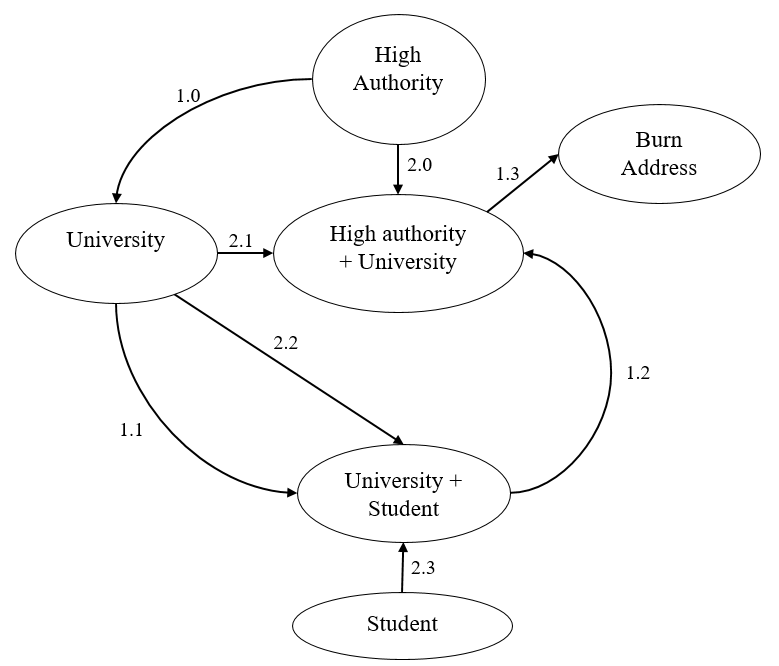
\includegraphics[width=\linewidth]{diplomaflow.png}
  \caption{Diploma issuance flow}
  \begin{tabular}{r@{: }l r@{: }l}
1.0& Transfer of asset with predetermined path to University\\ 
1.1& Transfer of asset to University-Student multisig wallet\\
1.2& Transfer of asset to H.A.-student multisig wallet \\
1.3& Transfer of asset to Burn Address\\
2.x& Consent to create multisignature address
\end{tabular}
\end{figure}

\subsection{Smart filters}

It should be said that the control filter used in this program is using the smart filter technology. The smart filter consists of a javascript code that runs every time a new transaction is  to be added to the blockchain. In our case the first High authority issues and approves the smart filter, which we included in the start script at the beginning of the blockchain. Once in place the filter works like this. Any transaction that is made from the university has to be to one of these addresses : the address embedded in the coin (which is the multisignature address between the high authority and university); an address without activate permission which is a student. Once the coin reaches a student-university multisignature it can be transferred only to the high-authority university multisignature.Once the asset reaches that moment the diploma is considered as issued. You can verify it by verifying the transaction trail left by the previous steps. Also when verifying a diploma one has to see if there is any revocation transaction which is represented by the transaction of the asset to the burn address.This can be initiated either by the high-authority or the university.
The flow of the diploma issuing process is illustrated in the figure below: 

\begin{figure}[h!]
  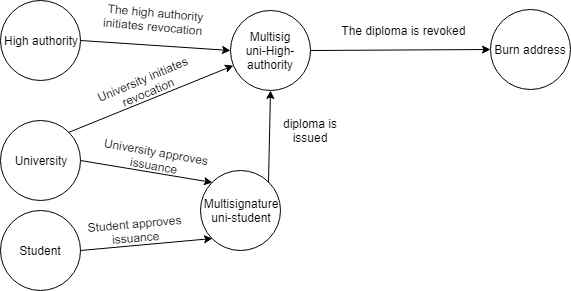
\includegraphics[width=\linewidth]{diploma.png}
  \caption{diploma issuance }
  \begin{tabular}{r@{: }l r@{: }l}
\end{tabular}
\end{figure}

\subsection{Diploma verification}

The next problem that we encounter is how does a certain company certify that a diploma belongs to an individual. There might be multiple individuals with the same name so the diploma hash is shared  will be the same for those individuals that went to the same universities and have the same name. We must insert the personal id number from the person that requests the diploma so that when a company verifies said diploma it can concatenate the id and the resulted hash is stored in the metadata of the coin when the diploma is issued. To sum up the company just verifies the existance of the one transaction from the university-student to the high authority multichain that signifies the issuance of the diploma . The second verification is about the absence of the second transaction which represents the revocation of the diploma. Using the hash of the diploma provided by the student. To this purpose we have given anyone connect permissions to the blockchain so that anyone can query the blockchain for information about diplomas making it a trivial operation to verify the authenticity of a certain diploma

\begin{figure}[h]
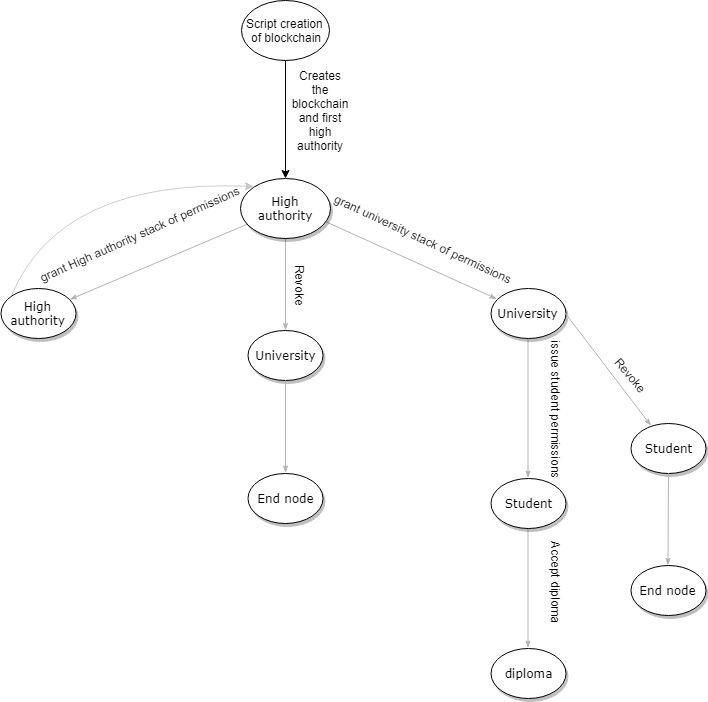
\includegraphics[width=\linewidth]{flow.png}
  \caption{The ecosystem of the entities }
\end{figure}





\section{Implementation}
We have used the multichain implementation to represent the system described below all code can be found at :..........<--link
In the first state we create the first high authority using a script. The first high authority also creates the blockchain . Any high authority has all permissions that are admissible by the multichain: connect; send ; receive ; issue ;create ; mine ; activate ; admin. This is state two. From this state the high authority can create universities and revoke them.\par
From the perspective of the high authority we can create multisignatures with the universities. This implies creating a shared wallet that can only spend the assets inside it with the approval of both members.The creation of the shared wallet is done separately from the university and from the high authority but the resulted wallet address is the same.\par
The high authority needs to grant the university some coins with it's address embedded in them so that the coins can only be transferred back to the university-high-authority multisignature address or to an address without activate permission . After the coin is generated the smart filter does not allow any transaction that will void the verification procedure. The coins are embedded by the university with the coin by appending them to the transaction. Then the student only needs to sign the transaction and it will be sent to the multisignature between the high authority and the university. Any attempt to send it to another address will result in the multichain declining the transaction. If there is any reason to retract said diploma it can be done either by the high-authority or by the university by initiating the process because the multisignature only needs one signature to send it to the burn address. Any attempt to send the transaction to another address will result in the transaction being declined.
If a third party wants to check the validity of a diploma or to verify what diplomas does a student have it can do this by getting the address of the student and then searching for all the transactions that the student did. Then we need to search if those transactions ended up in the burn address to see if the diplomas were revoked. In order to do this we verify the transactions of the assets if the asset has the provided diploma hash verify if the address of the transaction is the multisig between the high-authority and university and not the burn address. If it was sent to the burn address then the diploma is no longer valid.
For testing this implementation we strongly recommend the docker implementation we have included with the git hub project. For every entity that you want to use start as many dockers as you want.The instructions on how to start the dockers are included in the Readme. On the main machine you need to run the high authority because of the extra steps the high authority has to make and the fact that usually you only start one high authority. Then you start the dockers with the ports you want them mapped to and give them permission according to their respective rank. I have tested this implementation in an Ubuntu 18 virtual machine running 6 different entities. The new docker works by executing the dependency script like a normal user does and then it builds the local databases for both the university or high authority. If it is given permission it can function as any link in this blockchain. After everything is set up port 80 of the docker is exported which is then mapped to the port on the machine which is selected by the user.




\section{Hierarchical transfer}
The whole concept implemented by this model is referring to giving permission in accordance with your level in a certain hierarchy. The smart filter guides data circulation in a certain direction, making sure that it will end up in the wanted destination, then it does not concern itself with the other layers. All the layers will trust the upper layers and do not need to trust the lower layers because of the constraints given to them. For example The university is not trusted for the high authority so the high authority needs to set permissions accordingly in our scenario it gives the asset a metadata containing the return address . This is enforced by the smart filter implementation which will constrain all transactions with that certain coin to return to the high authority multisignature address. We find that this approach is both scalable and reliable because only one smart filter per level is attributed and also only one asset. In the model below we can see the permission:
\begin{figure}[h!]
  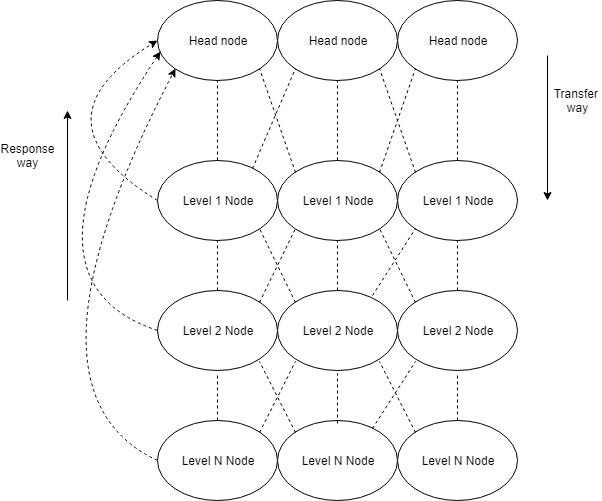
\includegraphics[width=\linewidth]{hierarchical.png}
  \caption{Hierarchical permission transfer flow}
  \begin{tabular}{r@{: }l r@{: }l}
\end{tabular}
\end{figure}

The head nodes can comunicate with all the level 1 nodes. We trust all head nodes as they control the transactions that go to the lower levels as well as the return address to when all the information or approval has been given to the asset. The first thing the head node does is to issue an asset with his return address issued to the level 1 node.\par In our implementation we needed that the university revoke the diploma too and with this purpose we created a common multisignature and put that address as the return address. After the asset is created the asset is given to the level 1 node. The level 1 can either transport the asset to a lower level node, which in our implementation was verified with the smart filters or back to the high authority.\par Each node can add it's own metadata to the transaction or just approve it. So for example we have a request from an institution and it needs to be signed by different people we can send that request to one of the people which represents the first level node and they will forward it to all the required nodes. We can also bypass all the unnecessary nodes but the sequence must be the same for example if we have the sequence 1 2 3 4 we can only do 1 3 4 but not 1 4 2 because of the permission hierarchy scheme.


%\section{Other possible uses}
%Other possible uses of this system are :
%\par
%Any system that requires a multi person acceptance to trigger a certain event.
%\par
%Any system that requires cert


\section{Security analysis}
In this section we will analyse the possibilities of attack from each perspective and we will list our defense mechanism for each of these.\par
1.The student is corrupt:\par
If the student is corrupt all he can do is not sign the diploma transfer in which case he does not get a diploma. He cannot harm the system as he only have send and receive permissions.\par
2.The university is corrupt:\par
If the university is corrupt it may try to send the diploma to another address except the high-authority but this is regulated with the help of smart filters. Our second defense mechanism is we can revoke the university rights from a High authority point of view. The university might also try to send the asset to the student directly but this does not constitute a diploma so it is not really a problem for the system it is treated like a spam transaction. For the last problem to be regulated we would have to put all addresses of multisignatures between the university and student to be written inside the asset and regulate it with another smart filter, but this solution is not scalable.\par
3.The high authority is corrupt:\par
From the perspective of a corrupt High authority you can do anything you want. We fully trust the ministry to remove only the untrusted universities and not interfere in the way the rules are being applied.
Also the high authority can send the asset directly to the student which will bypass the university but we also found the solution which is done at verification. We verify that the diploma was signed by an entity that has university like permissions. So with this last verification we can surely say that the university was accepted by the high authority and the diploma was issued by that university because the diploma is tied to the university signature

\section{Conclusions}
There are no any security problems that will disrupt this system. As stated above this is only one use of the hierarchical permissions, a system that we propose and will solve numerous problems that should require transparency and are currently  handled poorly by a centralized system. We can even restrict the path of the asset by specifying the which authorities it needs to get to for each step in the metadata of the asset.
The work implemented here can successfully withstand practical use and also it can be used for other purposes as well if the purpose of said application is to bind some kind of information to multiple lower tier entities like in the model described in the Hierarchical presentation above. Also this blockchain implementation helps us distribute the trust needed at each level so the high authority needs to trust the university and the university does not need to trust the student because the student is the bottom level of the hierarchical chain.


For our purpose we can only find that the blockchain is a perfect fit. We solve the trust issues between high authority and university and also the third party verification issues by using the transparency offered by the blockchain architecture.


Although multichain 2.0 has come a long way since it's early days it has still a lot of features to implement if it wants to boast about smart contracts.

We would like to add support for other diploma related actions as side-chains but the multichain architecture has not matured that much yet.
We would like to add the support to multiple smaller chains that could facilitate the accordance of certificates and maybe state issued ones like driver's id that would be tied to this chain but not influence it in any way.\par
We would like to implement some more security measures but the current state of the multichain implementation constrains us to only the ones we have implemented. Also we would like to simplify the verifying procedure but we would need the multichain api to evolve in order to do that.\par

\bibliographystyle{IEEEtran}
\bibliography{references}

\end{document}
